\documentclass[12pt,a4paper]{article}

\usepackage[utf8]{inputenc}
\usepackage[T1]{fontenc}
\usepackage[brazilian]{babel}
\usepackage{amsmath}
\usepackage{graphicx}
\usepackage{geometry}
\usepackage{float}
\usepackage{hyperref}
\usepackage{booktabs,tabularx,threeparttable,caption}

\geometry{top=2.5cm, bottom=2.5cm, left=3cm, right=3cm}

\title{Atividade 3: MLP \\ \large Disciplina: Redes Neurais Artificiais}
\author{Programa de Pós-Graduação em Ciência da Computação (PPGCC-UNESP)}
\date{\today}

\begin{document}

\maketitle

\section{Introdução e Implementação}
Este documento apresenta os resultados da implementação e avaliação do modelo MLP (Multilayer Perceptron). A MLP foi construída com o módulo de python conhecido como PyTorch, que provê implementações pré construídas importantes e otimizadas para GPU. Escolheu-se utilizar o DataLoader do Torch e uma arquitetura genérica para qualquer entrada, onde a rede deve identificar o tipo de problema de classificação (binário ou multiclasse), a partir dai definindo as funções de ativação ReLU ou Tahn, assim como o tamanho da camada final.

Como o CrossEntropy já aplica o softmax, o problema multiclasse é naturalmente resolvido, precisa-se apenas selecionar o argmax. No binário, é necessário ativar o vetor de 2 posições de saída, logo, pode-se usar a função sigmoid para ativar a saida do modelo e daí enviar para função BCELoss. Se usarmos a BCEWithLogitsLoss, esse sigmoid é automaticamente aplicado.

Utilizou-se o scikit\_learn para calcular-se as métricas, como f1\_score, AUC-ROC e acurácia. A sequência de testes foi estabelecida usando uma combinação entre conjuntos de arquiteturas, funções de ativação, datasets, otimizadores e tipos de regularização. Seguem exemplos dos treinos nessa estrutura.

\section{Experimentos no Dataset 1 e 2}

Os datasets 1 e 2 tinham uma natureza de classificação binária, o que se torna um problema trivial para uma MLP com até 3 camadas, o que, naturalmente, também gera um overfitting muito alto. Neste caso, não há nenhum problema nisso, pois os dados estão bem distribuidos e mesmo ao amostrar o dataset, os padrões permanecem. No entanto, num caso onde houvesse possível ruído, a mlp seria sobre treinada e retornaria resultados ruins para este problema bidimensional.

Abaixo, alguns exemplos de resultados:

\begin{figure}[H]
    \centering
    \begin{minipage}{0.48\textwidth}
        \centering
        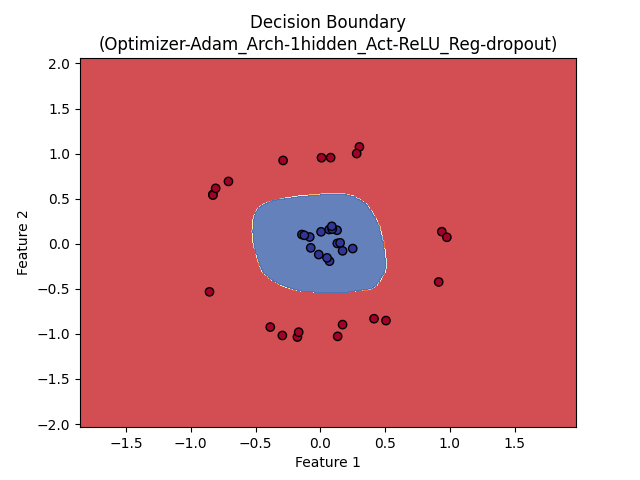
\includegraphics[width=\linewidth]{../../assets/mlp/Optimizer-Adam_Arch-1hidden_Act-ReLU_Reg-dropout_test_decision_boundary.png}
    \end{minipage}\hfill
    \begin{minipage}{0.48\textwidth}
        \centering
        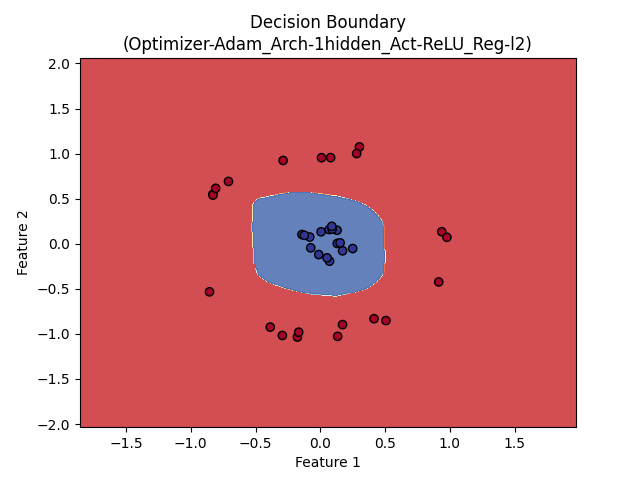
\includegraphics[width=\linewidth]{../../assets/mlp/Optimizer-Adam_Arch-1hidden_Act-ReLU_Reg-l2_test_decision_boundary.png}
    \end{minipage}
\end{figure}

Podemos ver os efeitos, no entanto, do overfitting supracitado nos dados de teste:

\begin{table}[h]
\centering
\caption{Resultados completos no conjunto de teste -- Dataset 1}
\label{tab:full_results_dataset_1}
\scriptsize
\setlength{\tabcolsep}{4pt}
\begin{tabular}{llllllllll}
\toprule
\textbf{Otim.} & \textbf{Arq.} & \textbf{Ativ.} & \textbf{Reg.} & \textbf{Loss} & \textbf{Acc} & \textbf{F1} & \textbf{AUC} & \textbf{Tr.Acc} & \textbf{Val.Acc} \\
\midrule
SGD & [2, 64, 1] & ReLU & none & 0.1659 & \textbf{0.9667} & \textbf{0.9666} & 0.9955 & \textbf{0.9857} & 0.9333 \\
SGD & [2, 64, 1] & ReLU & dropout & 0.1858 & \textbf{0.9667} & \textbf{0.9666} & 0.9955 & 0.9786 & 0.9333 \\
SGD & [2, 64, 1] & ReLU & l2 & 0.1532 & \textbf{0.9667} & \textbf{0.9666} & \textbf{1.0000} & \textbf{0.9857} & 0.9333 \\
SGD & [2, 64, 1] & Tanh & none & 0.1430 & \textbf{0.9667} & \textbf{0.9666} & 0.9955 & \textbf{0.9857} & 0.9333 \\
SGD & [2, 64, 1] & Tanh & dropout & 0.1576 & \textbf{0.9667} & \textbf{0.9666} & 0.9955 & 0.9786 & 0.9333 \\
SGD & [2, 64, 1] & Tanh & l2 & 0.1437 & \textbf{0.9667} & \textbf{0.9666} & 0.9955 & \textbf{0.9857} & 0.9333 \\
SGD & [2, 128, 64, 1] & ReLU & none & 0.1213 & \textbf{0.9667} & \textbf{0.9666} & \textbf{1.0000} & \textbf{0.9857} & 0.9333 \\
SGD & [2, 128, 64, 1] & ReLU & dropout & 0.1244 & \textbf{0.9667} & \textbf{0.9666} & \textbf{1.0000} & 0.9786 & 0.9333 \\
SGD & [2, 128, 64, 1] & ReLU & l2 & 0.1256 & \textbf{0.9667} & \textbf{0.9666} & \textbf{1.0000} & \textbf{0.9857} & 0.9333 \\
SGD & [2, 128, 64, 1] & Tanh & none & 0.1110 & \textbf{0.9667} & \textbf{0.9666} & 0.9955 & \textbf{0.9857} & 0.9333 \\
SGD & [2, 128, 64, 1] & Tanh & dropout & 0.1095 & \textbf{0.9667} & \textbf{0.9666} & 0.9955 & 0.9786 & 0.9333 \\
SGD & [2, 128, 64, 1] & Tanh & l2 & 0.1129 & \textbf{0.9667} & \textbf{0.9666} & 0.9955 & \textbf{0.9857} & 0.9333 \\
SGD & [2, 256, 128, 64, 1] & ReLU & none & 0.1070 & \textbf{0.9667} & \textbf{0.9666} & \textbf{1.0000} & \textbf{0.9857} & 0.9333 \\
SGD & [2, 256, 128, 64, 1] & ReLU & dropout & 0.1070 & \textbf{0.9667} & \textbf{0.9666} & \textbf{1.0000} & 0.9786 & 0.9333 \\
SGD & [2, 256, 128, 64, 1] & ReLU & l2 & 0.1180 & \textbf{0.9667} & \textbf{0.9666} & \textbf{1.0000} & \textbf{0.9857} & 0.9333 \\
SGD & [2, 256, 128, 64, 1] & Tanh & none & 0.1054 & \textbf{0.9667} & \textbf{0.9666} & 0.9955 & \textbf{0.9857} & 0.9333 \\
SGD & [2, 256, 128, 64, 1] & Tanh & dropout & 0.1086 & \textbf{0.9667} & \textbf{0.9666} & 0.9955 & \textbf{0.9857} & 0.9333 \\
SGD & [2, 256, 128, 64, 1] & Tanh & l2 & 0.1007 & \textbf{0.9667} & \textbf{0.9666} & 0.9955 & \textbf{0.9857} & 0.9333 \\
Adam & [2, 64, 1] & ReLU & none & 0.1051 & \textbf{0.9667} & \textbf{0.9666} & \textbf{1.0000} & \textbf{0.9857} & 0.9333 \\
Adam & [2, 64, 1] & ReLU & dropout & 0.1019 & \textbf{0.9667} & \textbf{0.9666} & \textbf{1.0000} & \textbf{0.9857} & 0.9333 \\
Adam & [2, 64, 1] & ReLU & l2 & 0.1009 & \textbf{0.9667} & \textbf{0.9666} & \textbf{1.0000} & \textbf{0.9857} & 0.9333 \\
Adam & [2, 64, 1] & Tanh & none & 0.1029 & \textbf{0.9667} & \textbf{0.9666} & 0.9955 & \textbf{0.9857} & 0.9333 \\
Adam & [2, 64, 1] & Tanh & dropout & 0.1044 & \textbf{0.9667} & \textbf{0.9666} & 0.9955 & 0.9786 & 0.9333 \\
Adam & [2, 64, 1] & Tanh & l2 & 0.1037 & \textbf{0.9667} & \textbf{0.9666} & 0.9955 & \textbf{0.9857} & 0.9333 \\
Adam & [2, 128, 64, 1] & ReLU & none & 0.0698 & \textbf{0.9667} & \textbf{0.9666} & \textbf{1.0000} & \textbf{0.9857} & 0.9333 \\
Adam & [2, 128, 64, 1] & ReLU & dropout & 0.0684 & \textbf{0.9667} & \textbf{0.9666} & \textbf{1.0000} & 0.9786 & 0.9333 \\
Adam & [2, 128, 64, 1] & ReLU & l2 & 0.0789 & \textbf{0.9667} & \textbf{0.9666} & \textbf{1.0000} & \textbf{0.9857} & 0.9333 \\
Adam & [2, 128, 64, 1] & Tanh & none & 0.1032 & \textbf{0.9667} & \textbf{0.9666} & \textbf{1.0000} & \textbf{0.9857} & 0.9333 \\
Adam & [2, 128, 64, 1] & Tanh & dropout & 0.1063 & \textbf{0.9667} & \textbf{0.9666} & \textbf{1.0000} & \textbf{0.9857} & 0.9333 \\
Adam & [2, 128, 64, 1] & Tanh & l2 & 0.0869 & \textbf{0.9667} & \textbf{0.9666} & \textbf{1.0000} & \textbf{0.9857} & 0.9333 \\
Adam & [2, 256, 128, 64, 1] & ReLU & none & 0.0581 & \textbf{0.9667} & \textbf{0.9666} & \textbf{1.0000} & \textbf{0.9857} & \textbf{0.9667} \\
Adam & [2, 256, 128, 64, 1] & ReLU & dropout & \textbf{0.0533} & \textbf{0.9667} & \textbf{0.9666} & \textbf{1.0000} & \textbf{0.9857} & 0.9333 \\
Adam & [2, 256, 128, 64, 1] & ReLU & l2 & 0.0665 & \textbf{0.9667} & \textbf{0.9666} & \textbf{1.0000} & \textbf{0.9857} & 0.9333 \\
Adam & [2, 256, 128, 64, 1] & Tanh & none & 0.0724 & \textbf{0.9667} & \textbf{0.9666} & \textbf{1.0000} & \textbf{0.9857} & 0.9333 \\
Adam & [2, 256, 128, 64, 1] & Tanh & dropout & 0.0885 & \textbf{0.9667} & \textbf{0.9666} & \textbf{1.0000} & \textbf{0.9857} & 0.9333 \\
Adam & [2, 256, 128, 64, 1] & Tanh & l2 & 0.0956 & \textbf{0.9667} & \textbf{0.9666} & \textbf{1.0000} & \textbf{0.9857} & 0.9333 \\
\bottomrule
\end{tabular}
\begin{tablenotes}
  \footnotesize
  \item Valores em \textbf{negrito} indicam o melhor resultado em cada métrica.
\end{tablenotes}
\end{table}


O mesmo se aplica para o dataset 2:

\begin{figure}[H]
    \centering
    \begin{minipage}{0.48\textwidth}
        \centering
        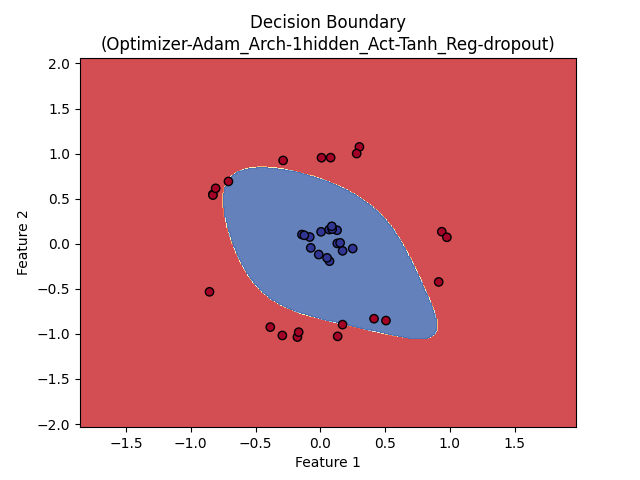
\includegraphics[width=\linewidth]{../../assets/mlp/Optimizer-Adam_Arch-1hidden_Act-Tanh_Reg-dropout_test_decision_boundary.png}
    \end{minipage}\hfill
    \begin{minipage}{0.48\textwidth}
        \centering
        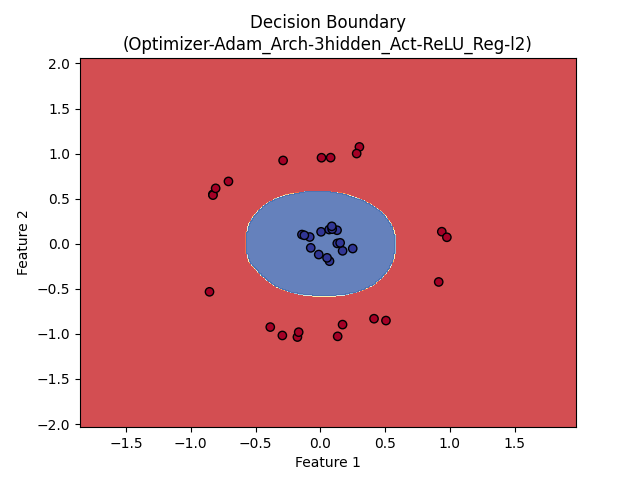
\includegraphics[width=\linewidth]{../../assets/mlp/Optimizer-Adam_Arch-3hidden_Act-ReLU_Reg-l2_test_decision_boundary.png}
    \end{minipage}
\end{figure}

\begin{table}[h]
\centering
\caption{Resultados completos no conjunto de teste -- Dataset 2}
\label{tab:full_results_dataset_2}
\scriptsize
\setlength{\tabcolsep}{4pt}
\begin{tabular}{llllllllll}
\toprule
\textbf{Otim.} & \textbf{Arq.} & \textbf{Ativ.} & \textbf{Reg.} & \textbf{Loss} & \textbf{Acc} & \textbf{F1} & \textbf{AUC} & \textbf{Tr.Acc} & \textbf{Val.Acc} \\
\midrule
SGD & [2, 64, 1] & ReLU & none & 0.4931 & \textbf{1.0000} & \textbf{1.0000} & \textbf{1.0000} & \textbf{1.0000} & \textbf{1.0000} \\
SGD & [2, 64, 1] & ReLU & dropout & 0.5876 & \textbf{1.0000} & \textbf{1.0000} & \textbf{1.0000} & 0.9371 & \textbf{1.0000} \\
SGD & [2, 64, 1] & ReLU & l2 & 0.5152 & 0.9730 & 0.9731 & \textbf{1.0000} & 0.9943 & 0.9737 \\
SGD & [2, 64, 1] & Tanh & none & 0.6738 & 0.6216 & 0.5846 & 0.6756 & 0.6857 & 0.6053 \\
SGD & [2, 64, 1] & Tanh & dropout & 0.6705 & 0.6757 & 0.6550 & 0.5952 & 0.6571 & 0.6842 \\
SGD & [2, 64, 1] & Tanh & l2 & 0.6718 & 0.6486 & 0.6206 & 0.7054 & 0.7257 & 0.6842 \\
SGD & [2, 128, 64, 1] & ReLU & none & 0.5308 & \textbf{1.0000} & \textbf{1.0000} & \textbf{1.0000} & \textbf{1.0000} & \textbf{1.0000} \\
SGD & [2, 128, 64, 1] & ReLU & dropout & 0.4344 & \textbf{1.0000} & \textbf{1.0000} & \textbf{1.0000} & \textbf{1.0000} & \textbf{1.0000} \\
SGD & [2, 128, 64, 1] & ReLU & l2 & 0.4101 & \textbf{1.0000} & \textbf{1.0000} & \textbf{1.0000} & \textbf{1.0000} & \textbf{1.0000} \\
SGD & [2, 128, 64, 1] & Tanh & none & 0.6492 & 0.6216 & 0.5846 & 0.8839 & 0.7086 & 0.6316 \\
SGD & [2, 128, 64, 1] & Tanh & dropout & 0.6615 & 0.5676 & 0.5066 & 0.9107 & 0.6514 & 0.5789 \\
SGD & [2, 128, 64, 1] & Tanh & l2 & 0.6724 & 0.6216 & 0.5846 & 0.5863 & 0.7200 & 0.6842 \\
SGD & [2, 256, 128, 64, 1] & ReLU & none & 0.4637 & \textbf{1.0000} & \textbf{1.0000} & \textbf{1.0000} & \textbf{1.0000} & \textbf{1.0000} \\
SGD & [2, 256, 128, 64, 1] & ReLU & dropout & 0.4781 & \textbf{1.0000} & \textbf{1.0000} & \textbf{1.0000} & \textbf{1.0000} & \textbf{1.0000} \\
SGD & [2, 256, 128, 64, 1] & ReLU & l2 & 0.4851 & \textbf{1.0000} & \textbf{1.0000} & \textbf{1.0000} & \textbf{1.0000} & \textbf{1.0000} \\
SGD & [2, 256, 128, 64, 1] & Tanh & none & 0.6749 & 0.6216 & 0.5846 & 0.6042 & 0.7200 & 0.6842 \\
SGD & [2, 256, 128, 64, 1] & Tanh & dropout & 0.6689 & 0.6216 & 0.5846 & 0.6071 & 0.7086 & 0.6842 \\
SGD & [2, 256, 128, 64, 1] & Tanh & l2 & 0.6592 & 0.6216 & 0.5846 & 0.6845 & 0.7143 & 0.6842 \\
Adam & [2, 64, 1] & ReLU & none & 0.0832 & \textbf{1.0000} & \textbf{1.0000} & \textbf{1.0000} & \textbf{1.0000} & \textbf{1.0000} \\
Adam & [2, 64, 1] & ReLU & dropout & 0.0975 & \textbf{1.0000} & \textbf{1.0000} & \textbf{1.0000} & \textbf{1.0000} & \textbf{1.0000} \\
Adam & [2, 64, 1] & ReLU & l2 & 0.1333 & \textbf{1.0000} & \textbf{1.0000} & \textbf{1.0000} & \textbf{1.0000} & \textbf{1.0000} \\
Adam & [2, 64, 1] & Tanh & none & 0.4761 & \textbf{1.0000} & \textbf{1.0000} & \textbf{1.0000} & 0.9943 & \textbf{1.0000} \\
Adam & [2, 64, 1] & Tanh & dropout & 0.4891 & 0.9189 & 0.9193 & \textbf{1.0000} & 0.9314 & 0.8947 \\
Adam & [2, 64, 1] & Tanh & l2 & 0.5393 & 0.8919 & 0.8922 & \textbf{1.0000} & 0.9657 & \textbf{1.0000} \\
Adam & [2, 128, 64, 1] & ReLU & none & 0.0007 & \textbf{1.0000} & \textbf{1.0000} & \textbf{1.0000} & \textbf{1.0000} & \textbf{1.0000} \\
Adam & [2, 128, 64, 1] & ReLU & dropout & 0.0005 & \textbf{1.0000} & \textbf{1.0000} & \textbf{1.0000} & \textbf{1.0000} & \textbf{1.0000} \\
Adam & [2, 128, 64, 1] & ReLU & l2 & 0.0041 & \textbf{1.0000} & \textbf{1.0000} & \textbf{1.0000} & \textbf{1.0000} & \textbf{1.0000} \\
Adam & [2, 128, 64, 1] & Tanh & none & 0.0076 & \textbf{1.0000} & \textbf{1.0000} & \textbf{1.0000} & \textbf{1.0000} & \textbf{1.0000} \\
Adam & [2, 128, 64, 1] & Tanh & dropout & 0.0142 & \textbf{1.0000} & \textbf{1.0000} & \textbf{1.0000} & \textbf{1.0000} & \textbf{1.0000} \\
Adam & [2, 128, 64, 1] & Tanh & l2 & 0.0158 & \textbf{1.0000} & \textbf{1.0000} & \textbf{1.0000} & \textbf{1.0000} & \textbf{1.0000} \\
Adam & [2, 256, 128, 64, 1] & ReLU & none & \textbf{0.0000} & \textbf{1.0000} & \textbf{1.0000} & \textbf{1.0000} & \textbf{1.0000} & \textbf{1.0000} \\
Adam & [2, 256, 128, 64, 1] & ReLU & dropout & \textbf{0.0000} & \textbf{1.0000} & \textbf{1.0000} & \textbf{1.0000} & \textbf{1.0000} & \textbf{1.0000} \\
Adam & [2, 256, 128, 64, 1] & ReLU & l2 & 0.0016 & \textbf{1.0000} & \textbf{1.0000} & \textbf{1.0000} & \textbf{1.0000} & \textbf{1.0000} \\
Adam & [2, 256, 128, 64, 1] & Tanh & none & 0.0007 & \textbf{1.0000} & \textbf{1.0000} & \textbf{1.0000} & \textbf{1.0000} & \textbf{1.0000} \\
Adam & [2, 256, 128, 64, 1] & Tanh & dropout & 0.0005 & \textbf{1.0000} & \textbf{1.0000} & \textbf{1.0000} & \textbf{1.0000} & \textbf{1.0000} \\
Adam & [2, 256, 128, 64, 1] & Tanh & l2 & 0.0046 & \textbf{1.0000} & \textbf{1.0000} & \textbf{1.0000} & \textbf{1.0000} & \textbf{1.0000} \\
\bottomrule
\end{tabular}
\begin{tablenotes}
  \footnotesize
  \item Valores em \textbf{negrito} indicam o melhor resultado em cada métrica.
\end{tablenotes}
\end{table}


Vemos que os resultados do datasets 2 estão no geral próximo a 1 com qualquer arquitetura com no mínimo 2 camadas escondidas e que o Adam se comportou muito bem para este dataset em especial, padrão que não será constatado no problema a seguir.

\section{Experimentos no Dataset 4}

O Dataset 4 é consideravelmente mais complexo, como pode ser visto nos resultdos a seguir, devido, mas não só à sua natureza multiclasse. Foram treinadas 100 épocas por arquitetura (com early stopping ativado), seguem os resultados:


\begin{table}[h]
\centering
\caption{Resultados completos no conjunto de teste -- Dataset 4}
\label{tab:full_results}
\scriptsize
\setlength{\tabcolsep}{4pt}
\begin{tabular}{llllllllll}
\toprule
\textbf{Otim.} & \textbf{Arq.} & \textbf{Ativ.} & \textbf{Reg.} &
\textbf{Loss} & \textbf{Acc} & \textbf{F1} & \textbf{AUC} &
\textbf{Tr.Acc} & \textbf{Val.Acc} \\
\midrule
SGD & [50, 64, 4] & ReLU & none & 0.5859 & 0.7917 & 0.7904 & \textbf{0.9483} & 0.9102 & 0.7812 \\
SGD & [50, 64, 4] & ReLU & dropout & \textbf{0.5822} & 0.7958 & 0.7959 & 0.9476 & 0.8893 & 0.8073 \\
SGD & [50, 64, 4] & ReLU & l2 & 0.5826 & 0.7958 & 0.7958 & 0.9453 & 0.8958 & 0.8021 \\
SGD & [50, 64, 4] & Tanh & none & 0.6021 & 0.8083 & 0.8092 & 0.9422 & 0.8529 & 0.7917 \\
SGD & [50, 64, 4] & Tanh & dropout & 0.5916 & 0.8083 & 0.8090 & 0.9439 & 0.8542 & 0.8073 \\
SGD & [50, 64, 4] & Tanh & l2 & 0.5912 & 0.8042 & 0.8040 & 0.9431 & 0.8568 & 0.7917 \\
SGD & [50, 128, 64, 4] & ReLU & none & 0.6052 & 0.7792 & 0.7796 & 0.9463 & 0.9245 & 0.7865 \\
SGD & [50, 128, 64, 4] & ReLU & dropout & 0.5903 & 0.7917 & 0.7919 & 0.9481 & 0.9102 & 0.7865 \\
SGD & [50, 128, 64, 4] & ReLU & l2 & 0.6045 & 0.7958 & 0.7953 & 0.9442 & 0.9102 & 0.7917 \\
SGD & [50, 128, 64, 4] & Tanh & none & 0.5950 & 0.7917 & 0.7918 & 0.9436 & 0.8594 & 0.8073 \\
SGD & [50, 128, 64, 4] & Tanh & dropout & 0.5984 & 0.7958 & 0.7954 & 0.9430 & 0.8490 & 0.7969 \\
SGD & [50, 128, 64, 4] & Tanh & l2 & 0.5837 & 0.8042 & 0.8046 & 0.9447 & 0.8542 & 0.8073 \\
SGD & [50, 256, 128, 64, 4] & ReLU & none & 0.6297 & \textbf{0.8167} & \textbf{0.8167} & 0.9463 & 0.9414 & 0.8073 \\
SGD & [50, 256, 128, 64, 4] & ReLU & dropout & 0.6177 & 0.8000 & 0.7993 & 0.9458 & 0.8958 & 0.7969 \\
SGD & [50, 256, 128, 64, 4] & ReLU & l2 & 0.6207 & 0.8125 & 0.8119 & 0.9453 & 0.9375 & 0.7708 \\
SGD & [50, 256, 128, 64, 4] & Tanh & none & 0.5946 & 0.8042 & 0.8042 & 0.9439 & 0.8594 & 0.8073 \\
SGD & [50, 256, 128, 64, 4] & Tanh & dropout & 0.5961 & 0.8042 & 0.8033 & 0.9433 & 0.8516 & 0.8125 \\
SGD & [50, 256, 128, 64, 4] & Tanh & l2 & 0.5907 & 0.8125 & 0.8130 & 0.9434 & 0.8542 & 0.7969 \\
Adam & [50, 64, 4] & ReLU & none & 0.7077 & 0.7625 & 0.7621 & 0.9402 & 0.9909 & 0.7552 \\
Adam & [50, 64, 4] & ReLU & dropout & 0.6557 & 0.7833 & 0.7826 & 0.9416 & 0.9688 & 0.7656 \\
Adam & [50, 64, 4] & ReLU & l2 & 0.6408 & 0.7875 & 0.7870 & 0.9450 & 0.9948 & 0.7604 \\
Adam & [50, 64, 4] & Tanh & none & 0.6668 & 0.7792 & 0.7785 & 0.9374 & 0.8958 & 0.7865 \\
Adam & [50, 64, 4] & Tanh & dropout & 0.6522 & 0.7792 & 0.7772 & 0.9414 & 0.8815 & 0.7969 \\
Adam & [50, 64, 4] & Tanh & l2 & 0.6564 & 0.7625 & 0.7615 & 0.9390 & 0.8945 & 0.7812 \\
Adam & [50, 128, 64, 4] & ReLU & none & 0.9396 & 0.7708 & 0.7698 & 0.9433 & 1.0000 & 0.7448 \\
Adam & [50, 128, 64, 4] & ReLU & dropout & 0.9494 & 0.7958 & 0.7948 & 0.9397 & 0.9948 & 0.7656 \\
Adam & [50, 128, 64, 4] & ReLU & l2 & 0.9169 & 0.7958 & 0.7943 & 0.9410 & 1.0000 & 0.7552 \\
Adam & [50, 128, 64, 4] & Tanh & none & 0.6737 & 0.7792 & 0.7779 & 0.9425 & 0.9492 & 0.7812 \\
Adam & [50, 128, 64, 4] & Tanh & dropout & 0.6681 & 0.7875 & 0.7883 & 0.9408 & 0.9062 & 0.8073 \\
Adam & [50, 128, 64, 4] & Tanh & l2 & 0.6750 & 0.7875 & 0.7870 & 0.9400 & 0.9297 & 0.7865 \\
Adam & [50, 256, 128, 64, 4] & ReLU & none & 1.3326 & 0.7750 & 0.7752 & 0.9354 & 1.0000 & 0.7917 \\
Adam & [50, 256, 128, 64, 4] & ReLU & dropout & 1.3325 & 0.7667 & 0.7644 & 0.9415 & 1.0000 & 0.7500 \\
Adam & [50, 256, 128, 64, 4] & ReLU & l2 & 1.1137 & 0.7708 & 0.7710 & 0.9407 & 1.0000 & 0.7500 \\
Adam & [50, 256, 128, 64, 4] & Tanh & none & 0.8093 & 0.8000 & 0.7994 & 0.9310 & 0.9870 & 0.7865 \\
Adam & [50, 256, 128, 64, 4] & Tanh & dropout & 0.8458 & 0.7833 & 0.7831 & 0.9280 & 0.9622 & 0.7760 \\
Adam & [50, 256, 128, 64, 4] & Tanh & l2 & 0.7506 & 0.7875 & 0.7859 & 0.9368 & 0.9805 & 0.7917 \\
\bottomrule
\end{tabular}
\begin{tablenotes}
  \footnotesize
  \item Valores em \textbf{negrito} indicam o melhor resultado em cada métrica.
\end{tablenotes}
\end{table}

\newpage

\subsection{Discussão}

Os 2 melhores resultados obtidos no dataset 4 não possuem nenhuma técnica de regularização, o que não necessariamente reflete um padrão. Haja vista que os melhores resultados de cada otimizador não estão exatamente na média dos resultados, o que demonstra que a regularização não obrigatoriamente melhora os resultados, mas, diminui consideravelmente o desvio padrão enquanto aumenta a média de resultados positivos. Observa-se que, diferentemente dos datasets binários anteriores, o uso do Adam em detrimento do SGD já não é mais lugar comum, agora, os resultados estão próximos e, na maioria dos testes, o SGD conseguiu resultados superiores ao Adam.

% TABLE 2 — Melhor por otimizador
\begin{table}[h]
\centering
\caption{Melhor configuração por otimizador (maior acurácia de teste)}
\label{tab:best_per_optimizer}
\begin{tabular}{llllllll}
\toprule
\textbf{Otim.} & \textbf{Arq.} & \textbf{Ativ.} & \textbf{Reg.} &
\textbf{Loss} & \textbf{Acc} & \textbf{F1} & \textbf{AUC} \\
\midrule
SGD & [50, 256, 128, 64, 4] & ReLU & none & 0.6297 & 0.8167 & 0.8167 & 0.9463 \\
Adam & [50, 256, 128, 64, 4] & Tanh & none & 0.8093 & 0.8000 & 0.7994 & 0.9310 \\
\bottomrule
\end{tabular}
\end{table}


% TABLE 3 — Impacto da regularização
\begin{table}[h]
\centering
\caption{Impacto da regularização (média $\pm$ desvio sobre todas as combinações)}
\label{tab:regularization}
\begin{tabular}{lllll}
\toprule
\textbf{Regularização} & \textbf{Acc ($\mu \pm \sigma$)} & \textbf{Loss ($\mu \pm \sigma$)} &
\textbf{F1 ($\mu$)} & \textbf{AUC ($\mu$)} \\
\midrule
Dropout ($p=0.1$) & 0.7910 $\pm$ 0.0116 & 0.7233 $\pm$ 0.2232 & 0.7904 & 0.9421 \\
L2 ($\lambda=0.001$) & \textbf{0.7930 $\pm$ 0.0152} & 0.6939 $\pm$ 0.1632 & 0.7926 & 0.9424 \\
Nenhuma & 0.7882 $\pm$ 0.0166 & 0.7285 $\pm$ 0.2175 & 0.7879 & 0.9417 \\
\bottomrule
\end{tabular}
\end{table}

Vê-se, como supracitado, que os valores médios tem uma significativa melhora com as regularizações propostas, mas que não necessariamente garantem o resltado ótimo.

\newpage

Ao analisar o gap\footnote{Gap $= \text{Tr.Acc} - \text{Val.Acc}$. Valores em \textbf{negrito} indicam gap $> 0.10$ (possível overfitting). \label{gap}}, é possível notar que o SGD possui, na média, um valor menor em comparação ao Adam. Ainda assim, é possível ver que com o gap consideravelmente alto pode  indicar um possível overfitting. A tabela \ref{tab:overfitting} apresenta os valores comparativos do gap.

% TABLE 4 — Análise de overfitting
\begin{table}[h]
\centering
\caption{Análise de overfitting: gap entre acurácia de treino e validação}
\label{tab:overfitting}
\scriptsize
\setlength{\tabcolsep}{4pt}
\begin{tabular}{llllllll}
\toprule
\textbf{Otim.} & \textbf{Arq.} & \textbf{Ativ.} & \textbf{Reg.} &
\textbf{Tr.Acc} & \textbf{Val.Acc} & \textbf{Ts.Acc} & \textbf{Gap\footref{gap}} \\
\midrule
Adam & [50, 128, 64, 4] & ReLU & none & 1.0000 & 0.7448 & 0.7708 & \textbf{0.2552} \\
Adam & [50, 256, 128, 64, 4] & ReLU & dropout & 1.0000 & 0.7500 & 0.7667 & \textbf{0.2500} \\
Adam & [50, 256, 128, 64, 4] & ReLU & l2 & 1.0000 & 0.7500 & 0.7708 & \textbf{0.2500} \\
Adam & [50, 128, 64, 4] & ReLU & l2 & 1.0000 & 0.7552 & 0.7958 & \textbf{0.2448} \\
Adam & [50, 64, 4] & ReLU & none & 0.9909 & 0.7552 & 0.7625 & \textbf{0.2357} \\
Adam & [50, 64, 4] & ReLU & l2 & 0.9948 & 0.7604 & 0.7875 & \textbf{0.2344} \\
Adam & [50, 128, 64, 4] & ReLU & dropout & 0.9948 & 0.7656 & 0.7958 & \textbf{0.2292} \\
Adam & [50, 256, 128, 64, 4] & ReLU & none & 1.0000 & 0.7917 & 0.7750 & \textbf{0.2083} \\
Adam & [50, 64, 4] & ReLU & dropout & 0.9688 & 0.7656 & 0.7833 & \textbf{0.2032} \\
Adam & [50, 256, 128, 64, 4] & Tanh & none & 0.9870 & 0.7865 & 0.8000 & \textbf{0.2005} \\
Adam & [50, 256, 128, 64, 4] & Tanh & l2 & 0.9805 & 0.7917 & 0.7875 & \textbf{0.1888} \\
Adam & [50, 256, 128, 64, 4] & Tanh & dropout & 0.9622 & 0.7760 & 0.7833 & \textbf{0.1862} \\
Adam & [50, 128, 64, 4] & Tanh & none & 0.9492 & 0.7812 & 0.7792 & \textbf{0.1680} \\
SGD & [50, 256, 128, 64, 4] & ReLU & l2 & 0.9375 & 0.7708 & 0.8125 & \textbf{0.1667} \\
Adam & [50, 128, 64, 4] & Tanh & l2 & 0.9297 & 0.7865 & 0.7875 & \textbf{0.1432} \\
SGD & [50, 128, 64, 4] & ReLU & none & 0.9245 & 0.7865 & 0.7792 & \textbf{0.1380} \\
SGD & [50, 256, 128, 64, 4] & ReLU & none & 0.9414 & 0.8073 & 0.8167 & \textbf{0.1341} \\
SGD & [50, 64, 4] & ReLU & none & 0.9102 & 0.7812 & 0.7917 & \textbf{0.1290} \\
SGD & [50, 128, 64, 4] & ReLU & dropout & 0.9102 & 0.7865 & 0.7917 & \textbf{0.1237} \\
SGD & [50, 128, 64, 4] & ReLU & l2 & 0.9102 & 0.7917 & 0.7958 & \textbf{0.1185} \\
Adam & [50, 64, 4] & Tanh & l2 & 0.8945 & 0.7812 & 0.7625 & \textbf{0.1133} \\
Adam & [50, 64, 4] & Tanh & none & 0.8958 & 0.7865 & 0.7792 & \textbf{0.1093} \\
Adam & [50, 128, 64, 4] & Tanh & dropout & 0.9062 & 0.8073 & 0.7875 & 0.0989 \\
SGD & [50, 256, 128, 64, 4] & ReLU & dropout & 0.8958 & 0.7969 & 0.8000 & 0.0989 \\
SGD & [50, 64, 4] & ReLU & l2 & 0.8958 & 0.8021 & 0.7958 & 0.0937 \\
Adam & [50, 64, 4] & Tanh & dropout & 0.8815 & 0.7969 & 0.7792 & 0.0846 \\
SGD & [50, 64, 4] & ReLU & dropout & 0.8893 & 0.8073 & 0.7958 & 0.0820 \\
SGD & [50, 64, 4] & Tanh & l2 & 0.8568 & 0.7917 & 0.8042 & 0.0651 \\
SGD & [50, 64, 4] & Tanh & none & 0.8529 & 0.7917 & 0.8083 & 0.0612 \\
SGD & [50, 256, 128, 64, 4] & Tanh & l2 & 0.8542 & 0.7969 & 0.8125 & 0.0573 \\
SGD & [50, 128, 64, 4] & Tanh & dropout & 0.8490 & 0.7969 & 0.7958 & 0.0521 \\
SGD & [50, 128, 64, 4] & Tanh & none & 0.8594 & 0.8073 & 0.7917 & 0.0521 \\
SGD & [50, 256, 128, 64, 4] & Tanh & none & 0.8594 & 0.8073 & 0.8042 & 0.0521 \\
SGD & [50, 64, 4] & Tanh & dropout & 0.8542 & 0.8073 & 0.8083 & 0.0469 \\
SGD & [50, 128, 64, 4] & Tanh & l2 & 0.8542 & 0.8073 & 0.8042 & 0.0469 \\
SGD & [50, 256, 128, 64, 4] & Tanh & dropout & 0.8516 & 0.8125 & 0.8042 & 0.0391 \\
\bottomrule
\end{tabular}
\end{table}


Pode-se observar na tabela \ref{tab:mean_results_activation}, em consonância, que as funções de ativação tem pouca diferença entre os resultados obtidos, sendo a acurácia da ReLU ou Tanh muita próximas no geral. 

\begin{table}[h]
\centering
\caption{Média das métricas por Função de Ativação -- Dataset 4}
\label{tab:mean_results_activation}
\scriptsize
\setlength{\tabcolsep}{4pt}
\begin{tabular}{lllllll}
\toprule
\textbf{Ativação} & \textbf{Loss} & \textbf{Acc} & \textbf{F1} & \textbf{AUC} & \textbf{Tr.Acc} & \textbf{Val.Acc} \\
\midrule
ReLU & 0.7782 & 0.7882 & 0.7877 & \textbf{0.9436} & \textbf{0.9536} & 0.7760 \\
Tanh & \textbf{0.6523} & \textbf{0.7933} & \textbf{0.7930} & 0.9404 & 0.8932 & \textbf{0.7952} \\
\bottomrule
\end{tabular}
\end{table}

\newpage
\section{Conclusão}
O dataset 4, em contraponto à simplicidade dos datasets 1 e 2, mostra que é difícil, mesmo para uma MLP, aproximar a função objetivo de maneira ótima. Os datasets menores e simples se tornam um problema trivial para a robustez de uma MLP. O mesmo não se aplica para datasets complexos, os quais serão abordados ao longo da disciplina, por isso vejo a necessidade (como esperado) de arquiteturas como CNN e Transformers. 

No geral, concluo o relatório respondendo as perguntas finais propostas na atividade

\textbf{Qual otimizador apresentou melhor estabilidade e desempenho.}
Adam é mais veloz para convergir, mas o SGD apresentou melhor generalização, o que bate com a literatura de ambos.

\textbf{Quais arquiteturas mostraram sinais de underfitting ou overfitting.}
O SGD, por ser estocástico, é menos estável e tende a apresentar possível underfitting. Ao combiná-lo com uma arquitetura menor, obtêm-se os piores resultados neste quesito. O overfitting é mais associado a arquitetura sem regularização.

\textbf{Qual estratégia de regularização foi mais eficaz.}
A regularização L2 teve uma média e desvio padrão melhores.

\textbf{Como a função de ativação influenciou os resultados.}
Menos do que eu esperava, ambas tiveram resultado similares.


\end{document}
